\chapter{Implementation}

Both Feeder and Explorer are implemented in Typescript and they are using js-ipfs\footnote{\url{https://github.com/ipfs/js-ipfs}} implementation of ipfs node. This allows code sharing between these two separated applications.

\section{Feeder implementation}
Informations about supported cryptocurrencies and enabled indexes are stored in Fedder's config file. Based on these settings, Feeder after start will begin to downloading data from Blockbook API, save them to IPFS, and create indexes of it.

\subsection{Indexes}
In my prototype, I tried a few different ways of indexing data in IPFS.
\begin{itemize}
    \item \textbf{OrbitDB}\footnote{\url{https://orbitdb.org/}} is a serverless, distributed, peer-to-peer database build on top of IPFS, developed by HAJA networks\footnote{\url{https://haja.io/}}. OrbitDB is good solution for small user's databases, but is is still in alpha stage of developing, and it is not well optimized to store hundreds gigabytes of data. The biggest problem is that OrbitDB performs all queries locally. To preform query like \texttt{db.query((tx) => tx.amount > 0.001)} OrbitDB needs to load all database locally and then cycling between them. So every client ends up with whole copy of database. This is not usable for our case, when we have database that has hundreds of gigabytes of data.
    \cite{OrbitDBManual}
    \item \textbf{Textile}\footnote{\url{https://textile.io/}} is a set of open source tools that provide a decentralized database, remote storage, user management, and more over the IPFS network. Textile already created applications for storing photos\footnote{\url{https://www.textile.photos/}}, notes\footnote{\url{https://noet.io/}} or anything else\footnote{\url{https://anytype.io/}}. Textile provides high abstraction on top of the IPFS and provides simple API to securely store and index files. It uses \textit{Cafe} peers to provides backups and indexing. Every data store is duplicated on several \textit{Cafe} peers. When client is obtaining some data, it will contact one of the \textit{Cafe} peers, and \textit{Cafe} peer will resolve query for the client. This is a problem for our solution, because using textile require lots of hardisk memory and does not solve problem with overloading \textit{Cafe} peers.
    \cite{TextileWhitePaper}
\end{itemize}

After some research, I came to conclusion that currently there is no solution for storing and indexing data in IPFS without high hardisk memory consumation. So I created my own indexing system that currently supports three types of index.

\begin{itemize}
    \item \textbf{Dictionary} - simple key-value structure that can be used for translating (for example block height to block). Search complexity is \texttt{O(1)} which is the fastest achievable speed. Big disadvantage is that client needs to download whole dictionary to performs search. In the time of writing this thesis, ethereum has 9 250 000 blocks. If we want to make dictionary for translating block height to IPFS block address, the size of this dictionary would be at least \texttt{(int\_size + multihash\_size) * 9 250 000 } where minimal size for \texttt{int\_size} is \texttt{4} bytes and \texttt{multihash\_size} is \texttt{36} bytes when sha-256 is used (32 bytes) and multihash prefix is 4 bytes long. So this dictionary would have over 1.3 GB only for ethereum. Another disadvantage is the impossibility to performing range search (for example get blocks between 9 249 950 and 2 500 000).
    \item \textbf{Reverse lookup} - This structure is inspired by DNS lookup\footnote{\url{https://en.wikipedia.org/wiki/Reverse_DNS_lookup}} and it's principle can be seen on figure \ref{reverseLookupIndex}.
    TODO opisat princíp. Key sa obrati atd.
\end{itemize}


\begin{figure}[H]
    \centering
    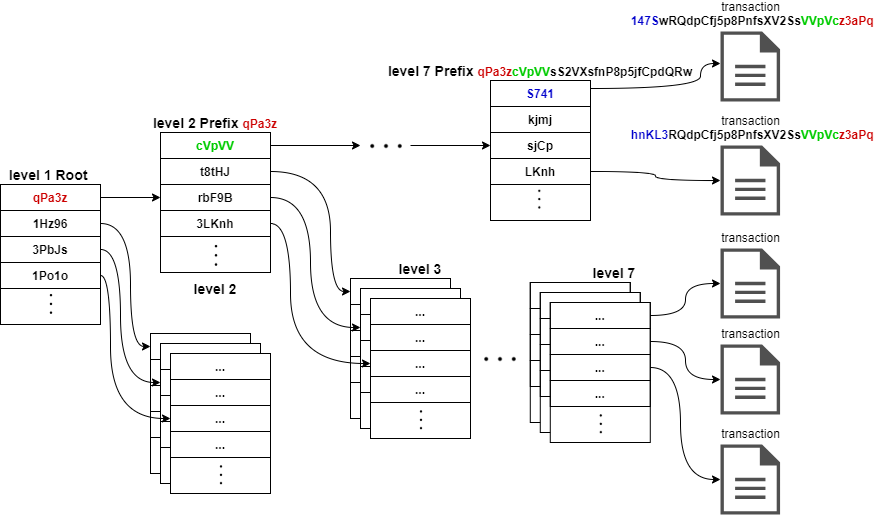
\includegraphics[width=13cm]{ReverseLookup_index.png}
    \caption{Reverse lookup by transaction hash}
    \label{reverseLookupIndex}
\end{figure}